\section{Results}
\label{sec:results-detail}

The per-paper hand-reviewed pilot samples previously shown here have been removed for
now, in favor of full-corpus aggregate results below, drawing on every paper classified
so far (Section~\ref{sec:extraction-classification}) rather than a small hand-picked
set.

\subsection{Full-corpus aggregate results (blueprint --- not yet finalized)}
\label{sec:results-aggregate}

Everything below draws on the full agent-classified corpus as classification proceeds,
generated by \texttt{plots/plots.ipynb}. This subsection is a placeholder skeleton, not
finished writing: every figure below is a candidate, not a commitment, and the
interpretive prose next to each one is a stub to be written once we decide what stays.
Every count is a snapshot from whenever the notebook was last run and will change as
classification continues; refresh the figures and re-check every number before treating
this as final.

\paragraph{Corpus size and classification status.} Table~\ref{tab:corpus-stats}
(Section~\ref{sec:corpus-size}) already reports this; repeated here only if a second
copy is useful right next to the results, otherwise cut.
% DECISION: keep here too, or rely on the existing Table~\ref{tab:corpus-stats}?

\begin{figure}[htbp]
\centering
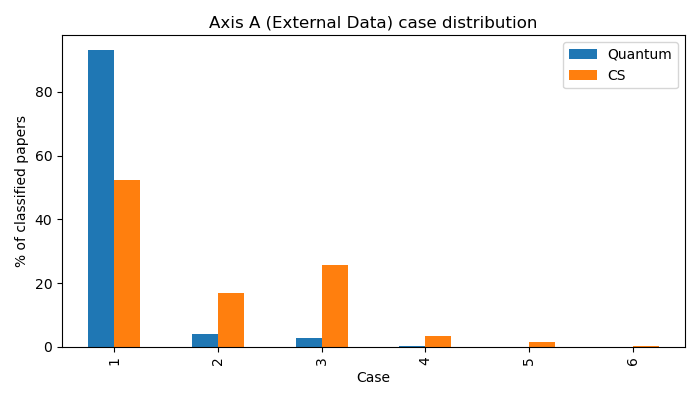
\includegraphics[width=0.85\textwidth]{plots/axis_a_distribution.png}
\caption{Axis A (External Data) case distribution, quantum vs.\ CS.}
\label{fig:axis-a-distribution}
\end{figure}
% DECISION: keep / cut / merge with Axis B below
[TBD: one to two sentences on what the Axis A split shows.]

\begin{figure}[htbp]
\centering
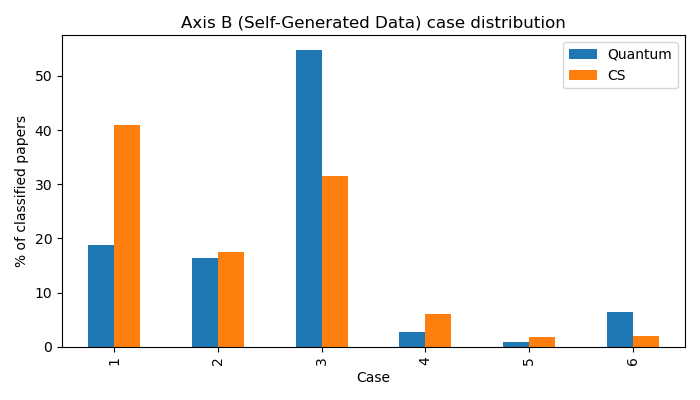
\includegraphics[width=0.85\textwidth]{plots/axis_b_distribution.png}
\caption{Axis B (Self-Generated Data) case distribution, quantum vs.\ CS.}
\label{fig:axis-b-distribution}
\end{figure}
% DECISION: keep / cut / merge with Axis A above
[TBD: one to two sentences on what the Axis B split shows.]

\begin{figure}[htbp]
\centering
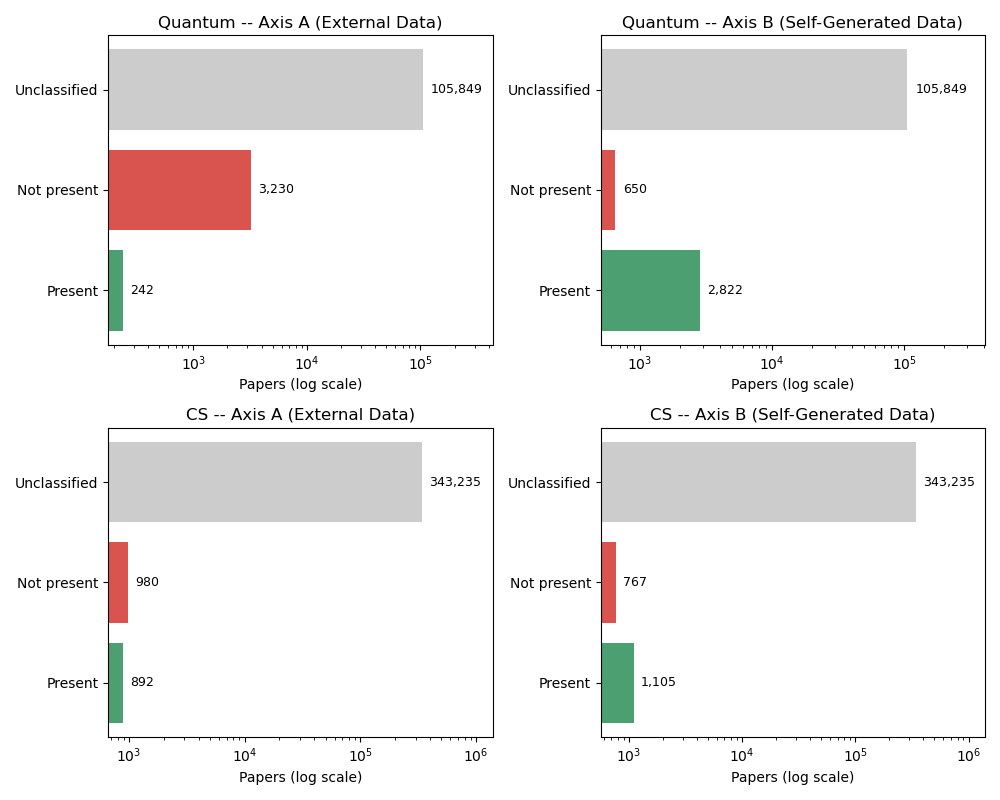
\includegraphics[width=0.85\textwidth]{plots/presence_vs_unclassified_bars.png}
\caption{Data present vs.\ not present vs.\ unclassified, per axis, per domain (full
corpus, log scale).}
\label{fig:presence-vs-unclassified}
\end{figure}
% DECISION: keep as a "how much is left" progress figure, or cut as more pipeline-status than result?
[TBD.]

\begin{table}[htbp]
\centering
\caption{Data present, by axis, per domain, out of that domain's classified papers so
far. Axis A = external data; Axis B = self-generated data; a paper can show data
present on either axis, both, or neither, so the two counts are independent and do not
sum to the classified total.}
\label{tab:present-by-axis-domain}
\begin{tabular}{@{}l r r r@{}}
\toprule
Domain & Classified & Axis A present & Axis B present \\
\midrule
CS & 1{,}872 & 892 & 1{,}105 \\
Quantum & 3{,}472 & 242 & 2{,}822 \\
\bottomrule
\end{tabular}
\end{table}
% DECISION: keep / cut -- overlaps with axis distribution figures above
[TBD.]

\begin{figure}[htbp]
\centering
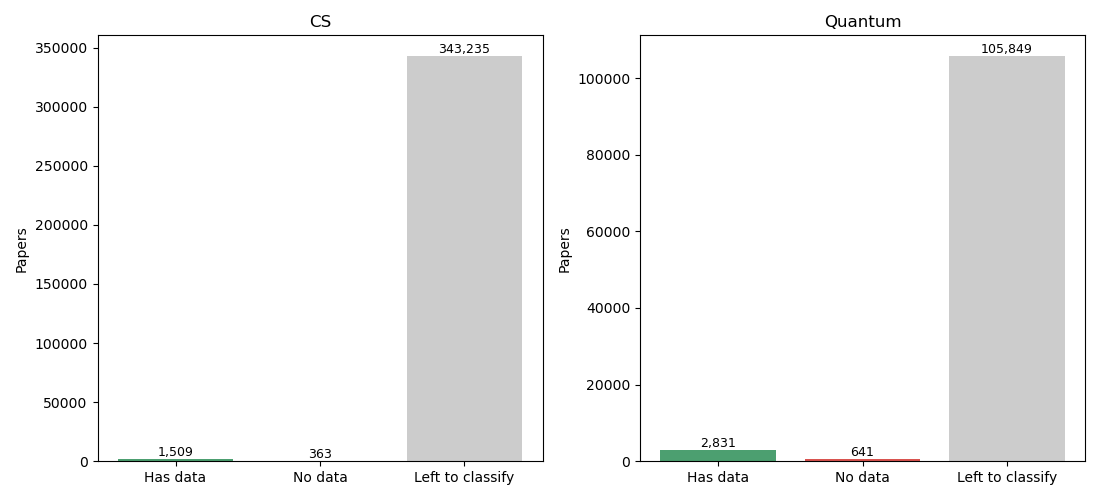
\includegraphics[width=0.85\textwidth]{plots/has_no_left_to_classify.png}
\caption{Has data vs.\ no data (theoretical) vs.\ left to classify, per domain (counts).}
\label{fig:has-no-left}
\end{figure}
% DECISION: keep counts version, pct version below, both, or neither (superseded by the funnel figures)?
[TBD.]

\begin{figure}[htbp]
\centering
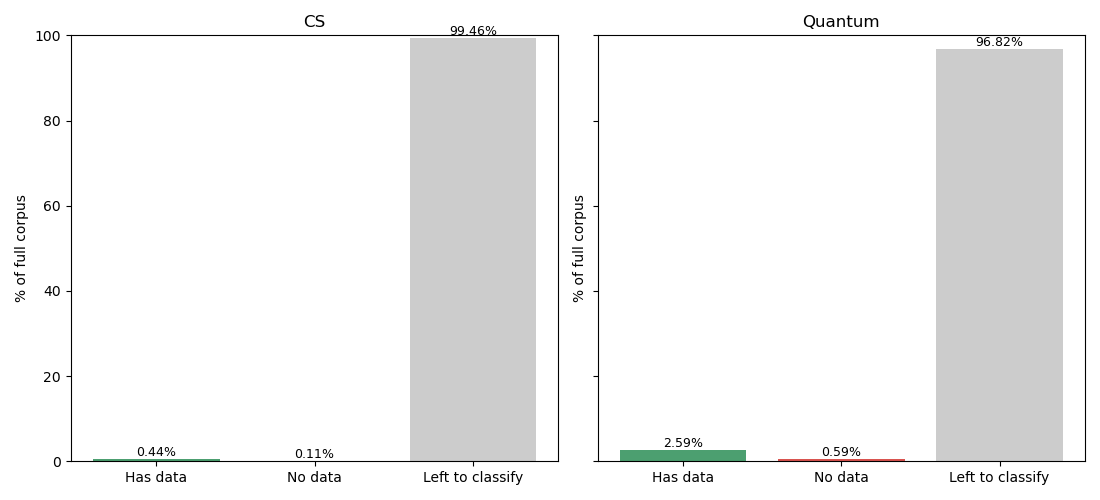
\includegraphics[width=0.85\textwidth]{plots/has_no_left_to_classify_pct.png}
\caption{Same breakdown as a percentage of each domain's full corpus.}
\label{fig:has-no-left-pct}
\end{figure}
% DECISION: keep / cut, see note above
[TBD.]

\begin{figure}[htbp]
\centering
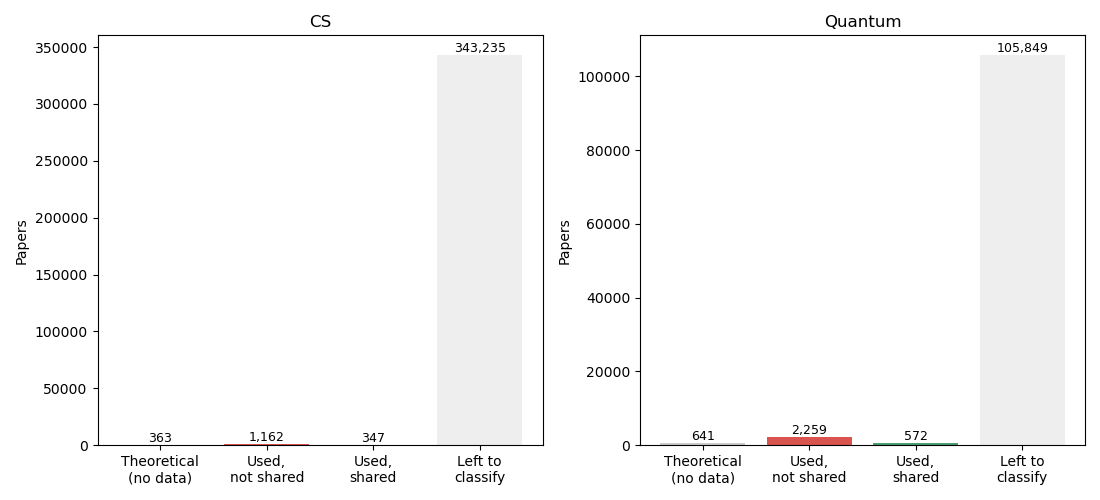
\includegraphics[width=0.85\textwidth]{plots/theoretical_shared_unshared.png}
\caption{Theoretical vs.\ used-but-not-shared vs.\ used-and-shared vs.\ left to
classify, per domain.}
\label{fig:theoretical-shared-unshared}
\end{figure}
% DECISION: likely a core figure -- candidate for the headline result of this section
[TBD.]

\begin{table}[htbp]
\centering
\caption{Shared vs.\ not shared, restricted to papers that use data at all (theoretical
papers -- Case 1 on both axes -- excluded, since they have no data to share in the
first place). ``Shared'' means every axis with data present is Case 2 (directly
accessible); ``not shared'' means at least one axis is Case 3, 4, 5, or 6.}
\label{tab:shared-vs-not-shared}
\begin{tabular}{@{}l r r r@{}}
\toprule
Domain & Papers using data & Shared & Not shared \\
\midrule
CS & 1{,}509 & 347 (23\%) & 1{,}162 (77\%) \\
Quantum & 2{,}831 & 572 (20\%) & 2{,}259 (80\%) \\
\bottomrule
\end{tabular}
\end{table}
% DECISION: likely a core table -- simplest, most direct statement of the comparison

\begin{table}[htbp]
\centering
\caption{Distribution of reasons data was not shared, pooled across both axes. A paper
whose two axes are unshared for two different reasons contributes to two cells here, so
each domain's row sums to more than that domain's ``Not shared'' count in
Table~\ref{tab:shared-vs-not-shared}. Case 3 = named/cited but no access path given at
all; Case 4 = acknowledged to exist but too vague to locate or reconstruct; Case 5 = a
specific link was given and does not resolve; Case 6 = available only on request, no
self-service path.}
\label{tab:not-shared-reasons}
\begin{tabular}{@{}l r r r r r@{}}
\toprule
Domain & Case 3 & Case 4 & Case 5 & Case 6 & Total \\
\midrule
CS & 1{,}070 (79\%) & 175 (13\%) & 63 (5\%) & 44 (3\%) & 1{,}352 \\
Quantum & 1{,}993 (85\%) & 111 (5\%) & 31 (1\%) & 221 (9\%) & 2{,}356 \\
\bottomrule
\end{tabular}
\end{table}
% DECISION: likely a core table -- shows *why* data goes unshared, not just that it does
[TBD.]

\begin{figure}[htbp]
\centering
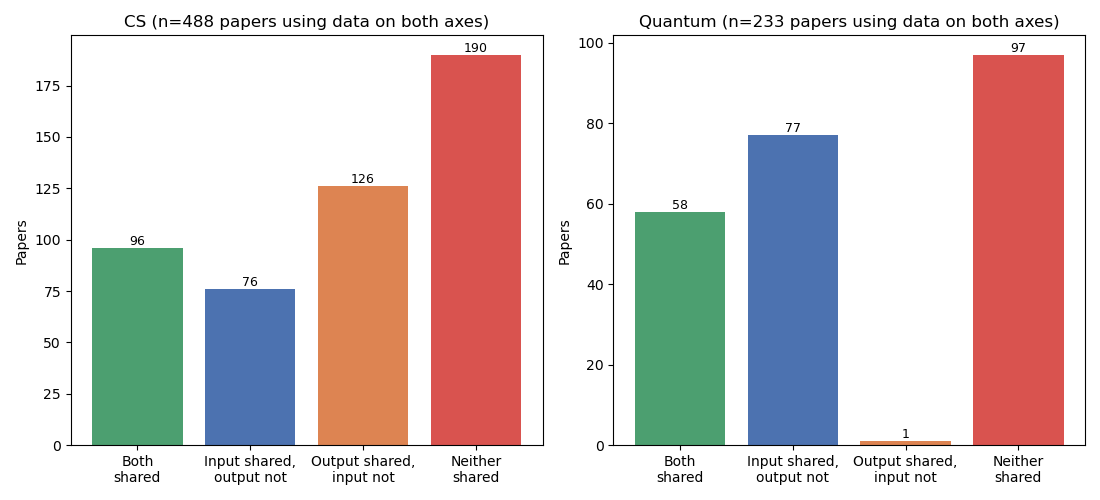
\includegraphics[width=0.85\textwidth]{plots/input_vs_output_shared.png}
\caption{Input shared vs.\ output shared, among papers using data on both axes (small
$n$ subset).}
\label{fig:input-vs-output-shared}
\end{figure}
% DECISION: keep as a secondary/appendix-style figure given the small n, or cut?
[TBD.]

\begin{figure}[htbp]
\centering
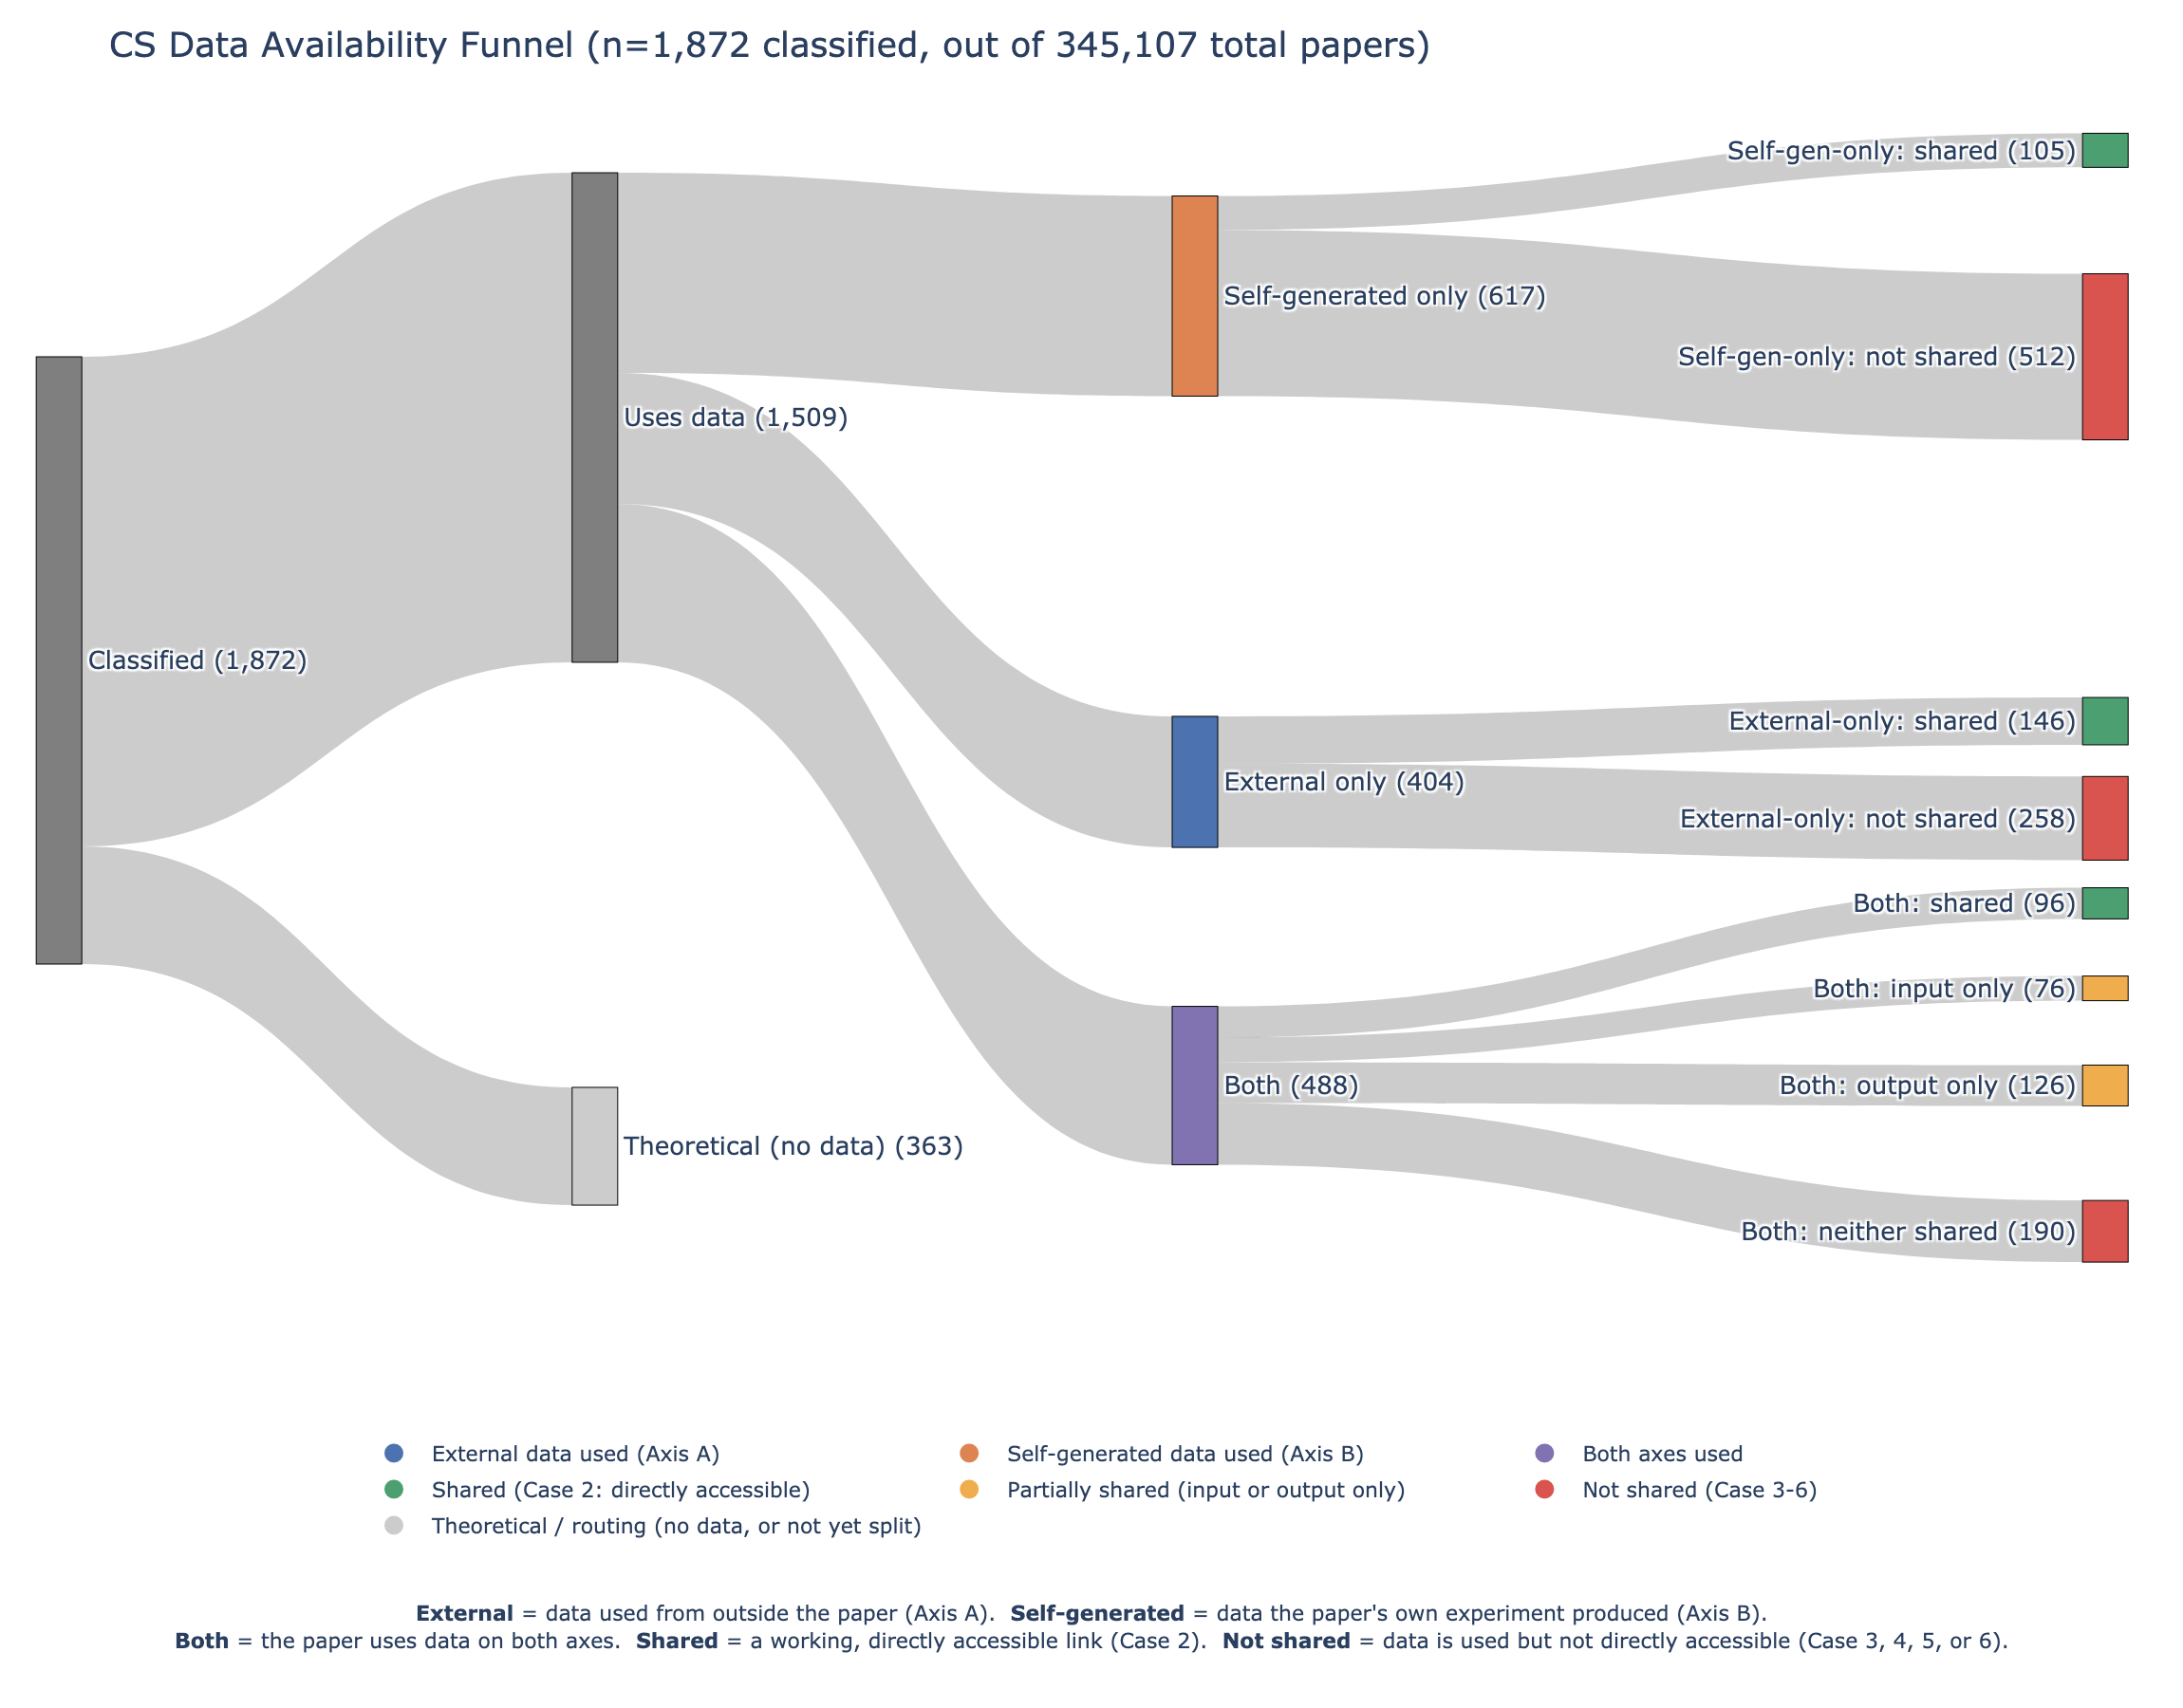
\includegraphics[width=\textwidth]{plots/funnel_cs.png}
\caption{Full funnel: uses data? which data? shared? --- CS.}
\label{fig:funnel-cs}
\end{figure}

\begin{figure}[htbp]
\centering
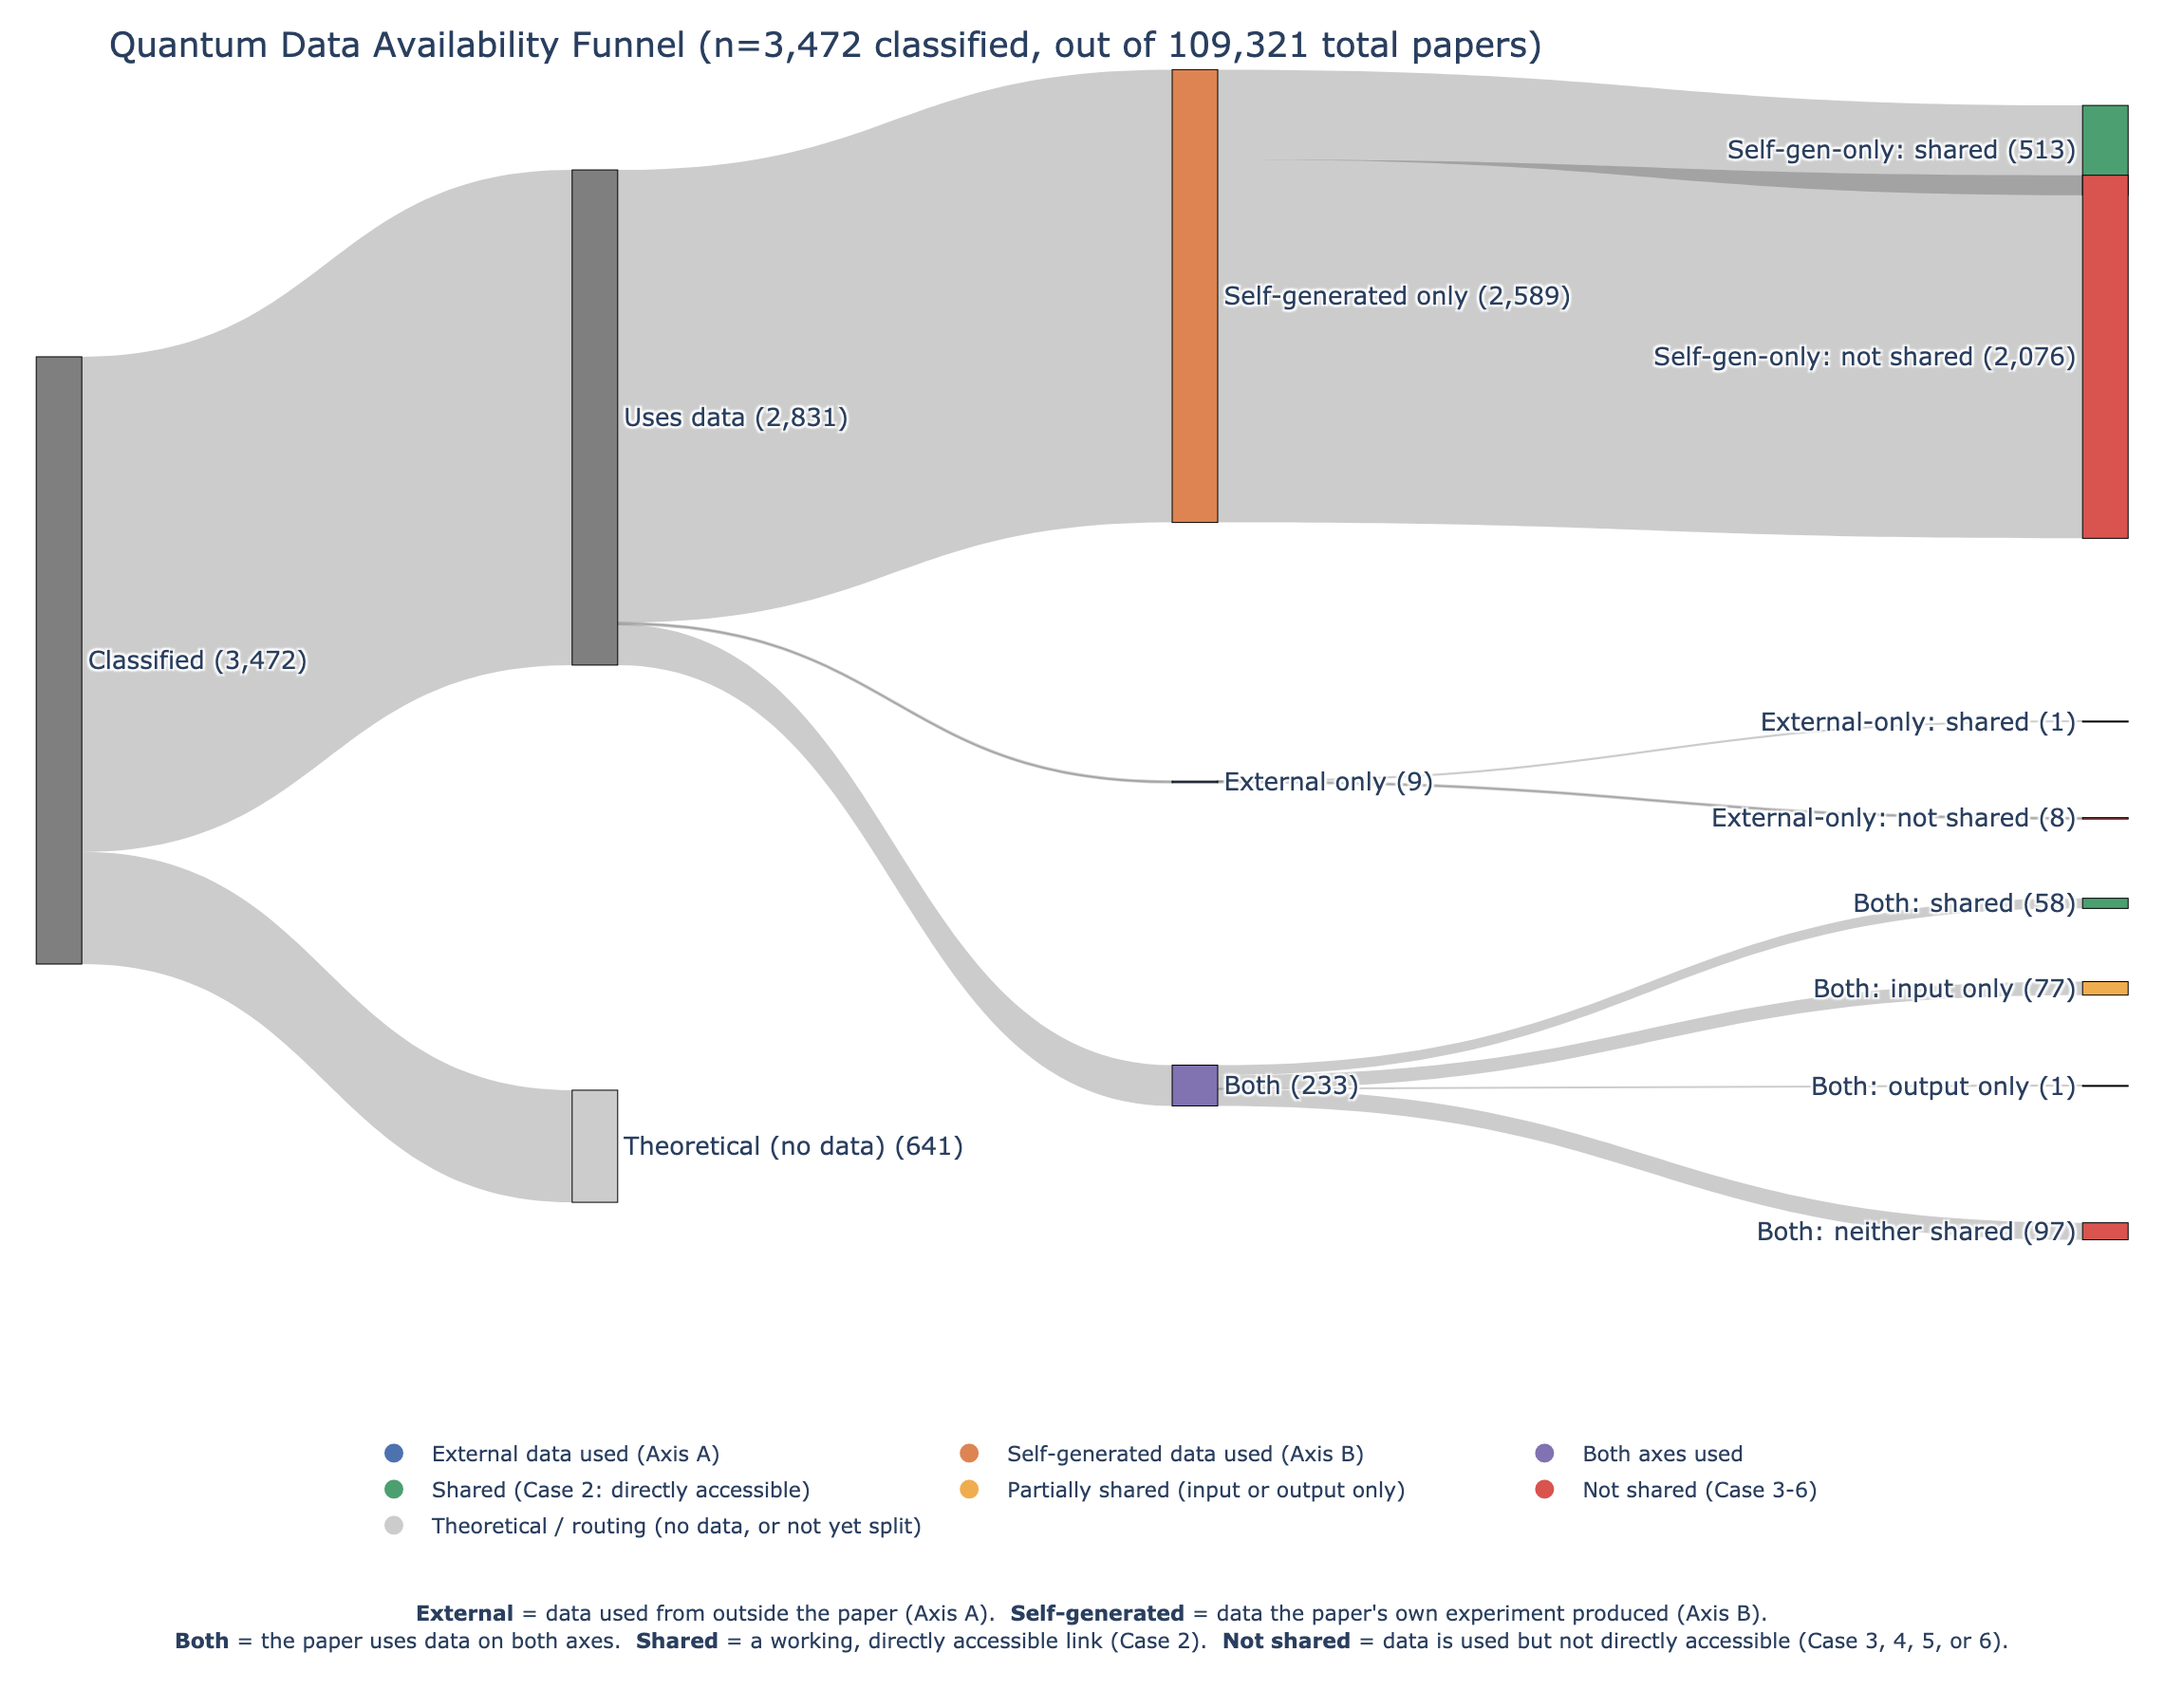
\includegraphics[width=\textwidth]{plots/funnel_quantum.png}
\caption{Full funnel: uses data? which data? shared? --- quantum.}
\label{fig:funnel-quantum}
\end{figure}
% DECISION: likely the single best summary figure per domain -- candidate to lead this
% section rather than close it; if so, move these two figures to the top.
[TBD.]
